\documentclass[twocolumn, a4paper]{UECIEresume}

\usepackage[dvipdfmx]{graphicx}
\usepackage{graphicx}
\usepackage{amsmath}
\usepackage{txfonts}

\title{対戦型パズルゲームにおける機械学習AIと人間の知識を用いたAIの比較}
\date{平成 29 年 2 月 14 日}
\affiliation{総合情報学科 メディア情報学 コース}
\supervisor{橋山智訓 准教授}
\studentid{1310163}
\author{柴澤弘樹}
%\headtitle{平成 yy 年度 総合情報学科 卒業論文中間発表}
\headtitle{平成 28 年度 総合情報学科 卒業論文発表}
%\headtitle{平成 yy 年度 総合情報学科 修士論文中間発表}
%\headtitle{平成 yy 年度 総合情報学科 修士論文発表}

\begin{document}
\maketitle

\section{序論}
近年のゲームAIの研究により、AIは人間と同等以上の強さを持つようになってきている。AlphaGo\cite{alphaGo}は囲碁で、DQN\cite{dqn}はAtari 2600のゲーム29種類で、それぞれ人間のプロプレイヤーを上回った。このような強さの背景には、ディープラーニングで評価関数を学習できるようになったことが大きく関わっている。

ディープラーニングでは、従来の人が設計していたものとは異なり、事前知識なしにゲームを学習できた。その汎用性の高さから、様々な問題に応用されている。一方で、学習の結果が分散して記録されるため、その解釈が困難であるデメリットが存在する。内部でどのような処理が行われているかはブラックボックスであり、学習結果が再利用できない。そのため、学習結果の確認やその改善には、多くの計算資源を費やしてトライアル&エラーを行うしかないのが現状である。

これまでのゲームAI研究は強さに着目して行われてきた。すべての情報がプレイヤーに対し開示されている完全情報ゲームの分野では、一定の成果が得られたといえる。しかし情報がプレイヤーから隠されている不完全情報ゲームについては、十分な研究がなされていない。商用ゲームのAIでは、開示されていないはずの情報を参照するなど、不公平感を生み出し楽しさを阻害してしまっている。

このような背景から、本研究では不完全情報ゲームにおいて人を楽しませるゲームAIの実装を目的とする。本稿ではその基礎的検討のために、対戦型パズルゲームである「ぷよぷよ」を対象とし、その対戦AIの実装を行う。ディープラーニングを用いたAIと人の知識を適用したAIの双方を実装することで、より優れた手法を検討し今後の研究指針とする。

\section{ぷよぷよのルール}
「ぷよぷよ」は落下型・対戦型パズルゲームの代表作であり、1991年の発売以後、現在に至るまで広く親しまれている。そのルールを簡単に説明する。

フィールドは横6マス縦13マスであり、ここに「ぷよ」と呼ばれる色ブロックを設置する。ぷよは2つが一組となってフィールドの上部から現れ、自然に落下してゆく。落下中は左右移動および左右回転ができ、任意の列か、隣り合った列にぷよを設置できる。落下予定のぷよは2手先まで表示されることから、現在の手を含めた3手分の情報が開示されている。一方でそれ以降の手は不明であり、ここに情報の不完全性が存在する。

設置後のぷよの下に空白マスがある場合、ぷよは下へ落下する。同色のぷよを4つ繋げると消すことができ、それによって空白が生まれた場合にはその上のぷよが落下する。落下後のぷよが同色で4つ以上つながる場合には再び消去が起こり、これが$n$回繰り返されることを$n$連鎖という。

対戦では連鎖の大きさに応じたスコアが計算される。プレイヤー間のスコアの差に応じて、おじゃまぷよを相手フィールドに降らすことができ、相手の連鎖構築を妨害できる。画面上部の左から3列目にぷよを設置するとゲームオーバーとなり、もう一方のプレイヤーが勝利する。

強いAIを実装するためには、連鎖を構築することが不可欠である。素早く大きな連鎖を組むために、不完全な情報から先の手を考慮した十分な先読みと柔軟さを行う事が求められる。今回の実装では連鎖威力、早さ、柔軟さの3要素を主眼に置き、これらを満たすAIによって強さを調べる。

\section{DQNによる戦術の学習}
DQN\cite{dqn}はディープラーニングとQ学習を組み合わせてゲームプレイを行うAIを構成する手法である。時刻$t$におけるゲーム画面を環境$s_t$、その時の操作を行動$a_t$として、それによって得られた次の時点$t+1$における報酬$R_{t+1}$から、評価関数$Q(s_t, a_t)$を更新する。

評価関数$Q(s_t, a_t)$はディープニューラルネットワークによって表現され、そのパラメータ$\theta_{t}$の更新式は以下の通りである。
\begin{eqnarray}
\theta_{t+1}(s_t, a_t) & = & \theta_t + \alpha (R_{t+1} + \gamma \max_a Q_t(s_{t+1}, a; \theta_t) \nonumber\\
& & - Q_t(s_t, a_t; \theta_t))\nabla_\theta Q_t(s_t, a_t; \theta_t)
\end{eqnarray}
ここで、$\alpha$は学習係数、$\gamma$は割引係数を表す。

%多くの試行によってゲームの状態と評価を学習でき、適切な操作を行うAIの実現に至った。Atari 2600のゲームでは48種類のゲームのうち43種類で従来のAIを上回り、29のゲームでプロの人間プレイヤーと同等以上のスコアを示した\cite{dqn}。さらにRLEを利用してスーパーファミコンのゲームを学習する試み\cite{RLE}も行われている。

DQNを「ぷよぷよ」のようなパズルゲームに適用した研究は未だなされていない。そこで今回は、スーパーファミコン版の「す〜ぱ〜ぷよぷよ通 リミックス」を用いて、ゲーム内AIとの対戦を通じた学習を行った。環境にはRLE\cite{RLE}を用い、学習ステップ数50000を100回繰り返した。報酬$R_{t+1}$は、(自スコア - 相手スコア)の時刻$t$から$t+1$での変化とした。

\section{人の知識を適用したAI}
\subsection{ポテンシャル最大化法}
従来のぷよぷよAIにおいて、基礎的な連鎖構築アルゴリズムとしてポテンシャル最大化法が比較対象とされてきた\cite{puyo_monte, puyo_temp}。その手続きは、以下の通りである。
\begin{enumerate}
\item 3手先までの配置可能な手および盤面を全て列挙する。
\item 1手目でぷよを消去する手を除外する。
\item 2手目、3手目で連鎖を発火したとき、スコアが最大となる手を選択する。ただし、候補手が複数ある場合には、その中からランダムに選択する。
\item 選択された手に至る1手目を、現在のツモの配置として決定する。
\end{enumerate}

開示されている手に関する全探索を行い、人が定めた評価を用いて最適手を選択する手法となっている。評価方法については、モンテカルロ法を用いた研究\cite{puyo_monte}で検討されている。しかし、探索方法と最適手の選択に関する研究は未だ十分なものではなく、改良の余地があると考えられる。そのため、まず3手目を開示された手のみに限らず全幅探索とし、またぷよを消去する手も探索に含める改良を行った。

\subsection{人の知識の適用}
人が評価を定めた探索手法であるポテンシャル最大化法に、さらに人の知識を加えた対戦用AIの実装を行った。知識は基礎的連鎖である3-1階段を構築するための手順を、if--thenルールによって記述したものである。この手順をゲーム開始直後の6手分用い、その後に改良した連鎖ポテンシャル法を用いることで、構築連鎖数の安定化を図った。

また対戦のために、構築した連鎖が閾値として定めた威力以上で発動できるとき、即座に発動する戦術をとった。閾値は4連鎖相当である、2100点に設定した。このような単純なルールベースAIを用いて、連鎖構築能力と対戦における強さを調べた。

\subsection{連鎖構築シミュレーション}
ポテンシャル最大化法の変更に伴う改善効果を検証するため、シミュレーションによって構築連鎖数を調べた。手数は32手で連鎖を構築し、33手目に任意の着手で発火するものとした。試行回数は50回とし、すべてのシミュレーションで同じ配石を用いた。

従来のポテンシャル最大化法、探索手法改善による方法、人の知識を適用した手法によるそれぞれの構築連鎖数の分布を、図\ref{fig:chain}に示す。探索方法の変更によって連鎖数が大きく改善され、人の知識を適用することでそのさらなる安定化に成功した。人の知識を適用したAIでは、配石をより適切に配置し、柔軟で効率的な連鎖を構築できることがわかった。また探索における1手あたりの平均計算時間は53.82 msであり、十分な早さで大きな威力の連鎖を構築できたと考えられる。

\begin{figure}[htb]
  \begin{center}
  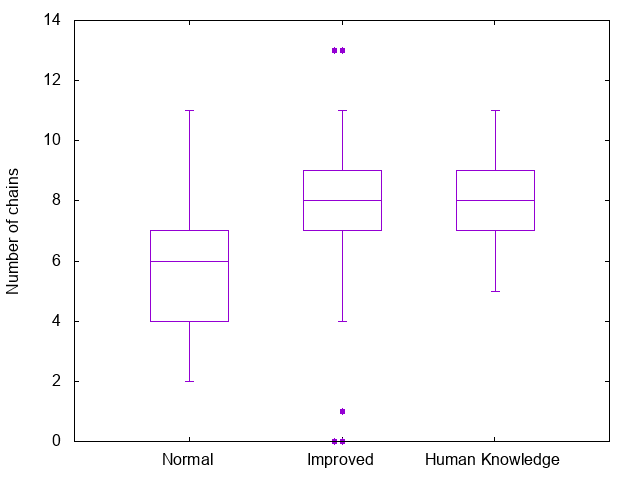
\includegraphics[height=5cm]{../graph/chain.png}
  \caption{ポテンシャル法の改良法と人の知識を適用したAIによる連鎖構築} \label{fig:chain}
\end{center}
\end{figure}

\section{ゲーム内AIとの対戦}
DQNによって対戦の戦術を学習したAIと、人の知識をルールベースで適用したAIについて、それぞれゲーム内のAIとの対戦成績による強さの比較を行った。対象とするゲームはスーパーファミコンの「す〜ぱ〜ぷよぷよ通 リミックス」、敵AIは「のほほ」とした。%「のほほ」はぷよを左端から高速で積み上げ、それを崩すことで連鎖を狙う。時として5連鎖以上をも放つ上に、3列目にはあまりぷよを設置しないことからフィールドが埋まりにくく、ゲームの中で最も強いAIの一つである。

それぞれ「のほほ」との50戦を行い、その勝敗とスコアを調べた。結果を表\ref{tab:win}、表\ref{tab:score}に示す。DQNは時として5連鎖を発動するに至るまで学習が進んだが、強さでは圧倒的に劣っていた。一方の人の知識を適用したAIでは、単純なルールであったにも関わらず「のほほ」とほぼ対等の強さを誇り、スコアでは上回った。さらに戦術面に関する知識を補強できる余地があり、人の知識を基にするAIはさらに強くなる可能性を秘めている。


\begin{table}[tbp]
\begin{center}
\caption{実装AIと「のほほ」との対戦における勝利数} \label{tab:win}
  \begin{tabular}{|l|c|c|} \hline
アルゴリズム & 実装AI & のほほ\\ \hline
DQN & 2 & 48\\ \hline
人の知識を適用したAI & 24 & 26\\ \hline
\end{tabular}
\end{center}
\end{table}


\begin{table}[tbp]
\begin{center}
\caption{実装AIと「のほほ」との対戦における平均スコア} \label{tab:score}
  \begin{tabular}{|l|c|c|} \hline
アルゴリズム & 実装AI & のほほ\\ \hline
DQN & 743.30 & 1790.12\\ \hline
人の知識を適用したAI & 4762.52 & 2703.74\\ \hline
\end{tabular}
\end{center}
\end{table}


\section{結論}
本稿では、機械学習によるAIと人の知識を適用したAIの双方を実装し、対戦型パズルゲームの「ぷよぷよ」においてその強さを評価した。機械学習の手法としてDQNを用いたAIでは50試合中2勝に留まったのに対し、人の知識を適用したAIでは24勝を収めることができた。よって現状では人の知識を用いたAIが、不完全情報ゲームの一つである「ぷよぷよ」では有効であったと結論づけた。

機械学習によるAIは学習方法を変えることで、人の知識を基にしたAIでは戦術に関する知識を補強することで、さらなる強さを獲得できる可能性がある。しかし、機械学習では学習内容の解釈が困難であるために改良が難しく、人の知識の適用ではその形式化が難しい。今後はこれらを組み合わせることで、より効率的な学習を行い、強さを向上させることを目指す。

{\small
\bibliographystyle{jplain}
\bibliography{../../ref}
}
\end{document}
